\documentclass{article}

\usepackage{graphicx} % for images
\usepackage{amsmath} % for math
\usepackage{amssymb} % for \mathbb
\usepackage{siunitx} % for \SI, \num
\usepackage{hyperref} % for \url{}

% This stuff is for figures
\usepackage{float}
\DeclareGraphicsExtensions{.pdf, .png, .jpg}

% coloring of links for PDF format
\hypersetup{
    colorlinks=true,
    urlcolor=blue,
    linkcolor=black
}

% \c command redefinition (for monospaced font)
\renewcommand{\c}[1]{\texttt{#1}}
% \today command re-definition
%https://tex.stackexchange.com/questions/112932/today-month-as-text
\renewcommand{\today}{\ifnum\number\day<10 0\fi \number\day \space%
\ifcase \month \or January\or February\or March\or April\or May%
\or June\or July\or August\or September\or October\or November\or December\fi\space%
\number \year} 

\begin{document}

\noindent
Rodrigo Becerril Ferreyra\\
E E 381 Section 12\\
Lab 6\\
\today

\addcontentsline{toc}{section}{Introduction}
\section*{Introduction} The purpose of this lab is to
put our knowledge of Markov chains into practice. Markov
chains are used to represent sequences.

\section{Problem 1}
In this problem, a Markov chain was experimentally tested
to see if it converges, and it was compared with the
expected, calculated values. Figure
\ref{plot:expected vs actual} shows the expected progression
of the Markov chain (probability of the given Markov chain vs
the iteration) compared to the acquired values obtained by
running the Markov chain \num{10000} times. Figure
\ref{plot:single run} shows one single run of a Markov chain,
plotted as state number vs iteration.

\begin{figure}[H]
    \centering
    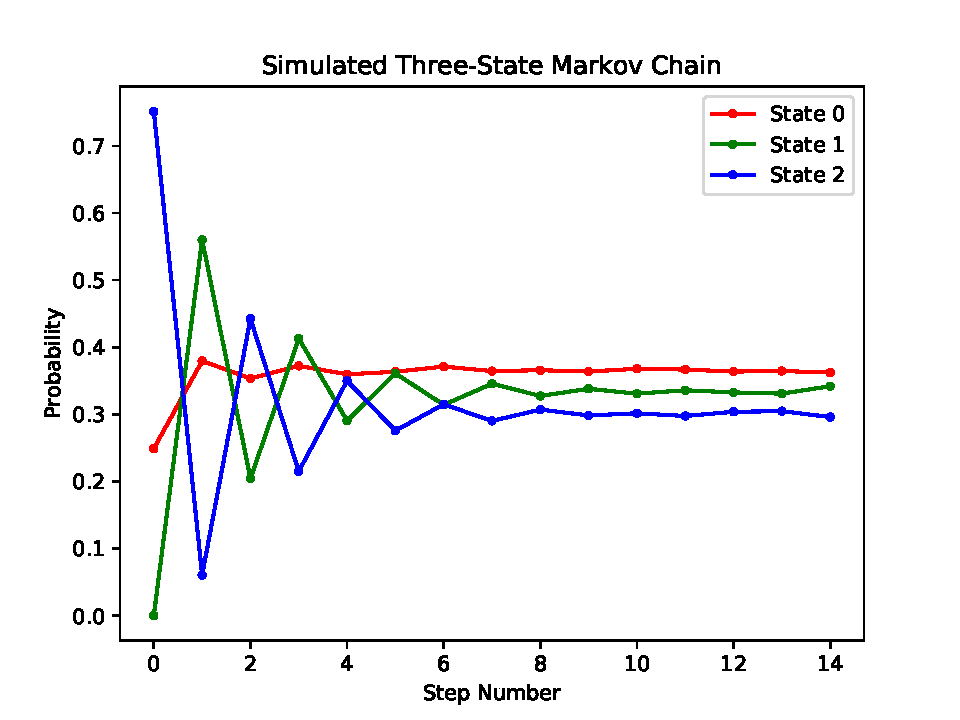
\includegraphics[width=0.49\textwidth]{Images/Problem1Figure2}
    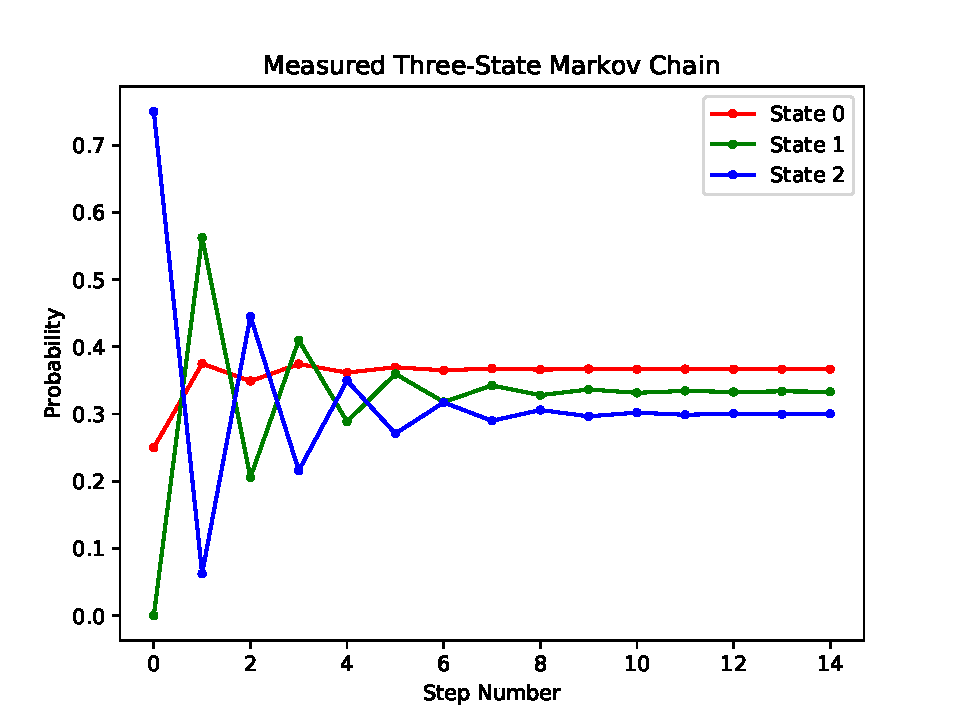
\includegraphics[width=0.49\textwidth]{Images/Problem1Figure3}
    \caption{Expected vs actual Markov Chain Progression.}
    \label{plot:expected vs actual}
\end{figure}
\begin{figure}[H]
    \centering
    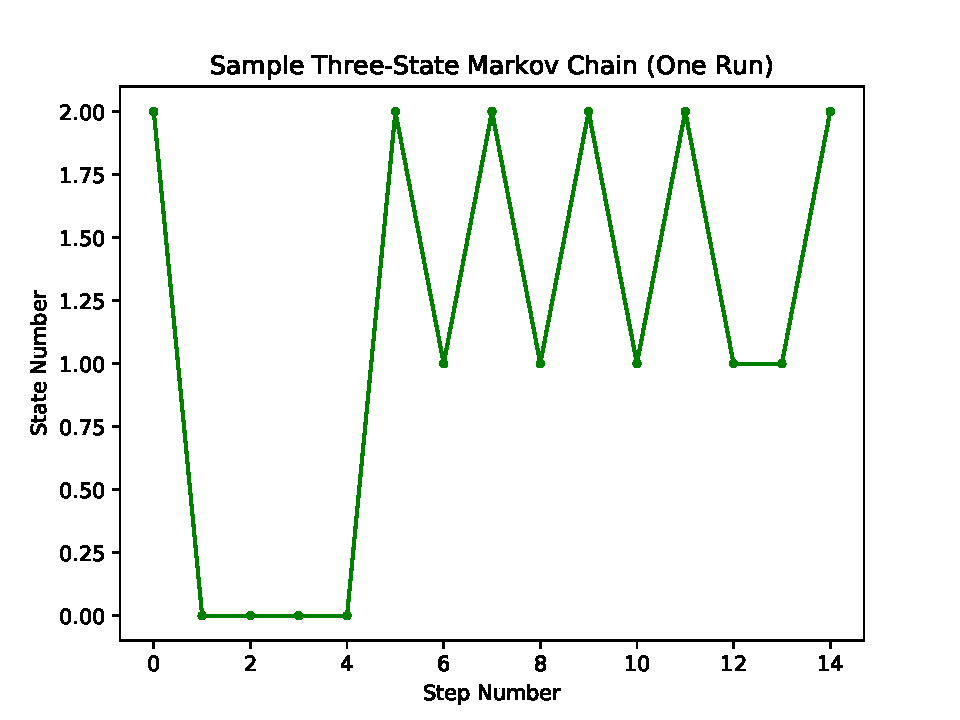
\includegraphics[width=0.49\textwidth]{Images/Problem1Figure1}
    \caption{A single Markov chain.}
    \label{plot:single run}
\end{figure}

\section{Problem 2}
In this problem, we were asked to use a simplified version
of Google's PageRank algorithm to rank five webpages given a
diagram of links. This was done twice: once where each of the
five pages have the same probability of being first, and
once where Page E was the initial state. In both cases,
the pages were ranked as follows:
\begin{enumerate}
    \item B
    \item A
    \item C
    \item E
    \item D
\end{enumerate}

This was regardless of the initial state vector. The following
matrix shows the Markov state probability table.

\begin{equation*}
    \begin{bmatrix}
        0 & 1 & 0 & 0 & 0\\
        1/2 & 0 & 1/2 & 0 & 0 \\
        1/3 & 1/3 & 0 & 0 & 1/3 \\
        1 & 0 & 0 & 0 & 0\\
        0 & 1/3 & 1/3 & 1/3 & 0
    \end{bmatrix}
\end{equation*}

Below are the plots showing the progression of the
Markov chain.

\begin{figure}[H]
    \centering
    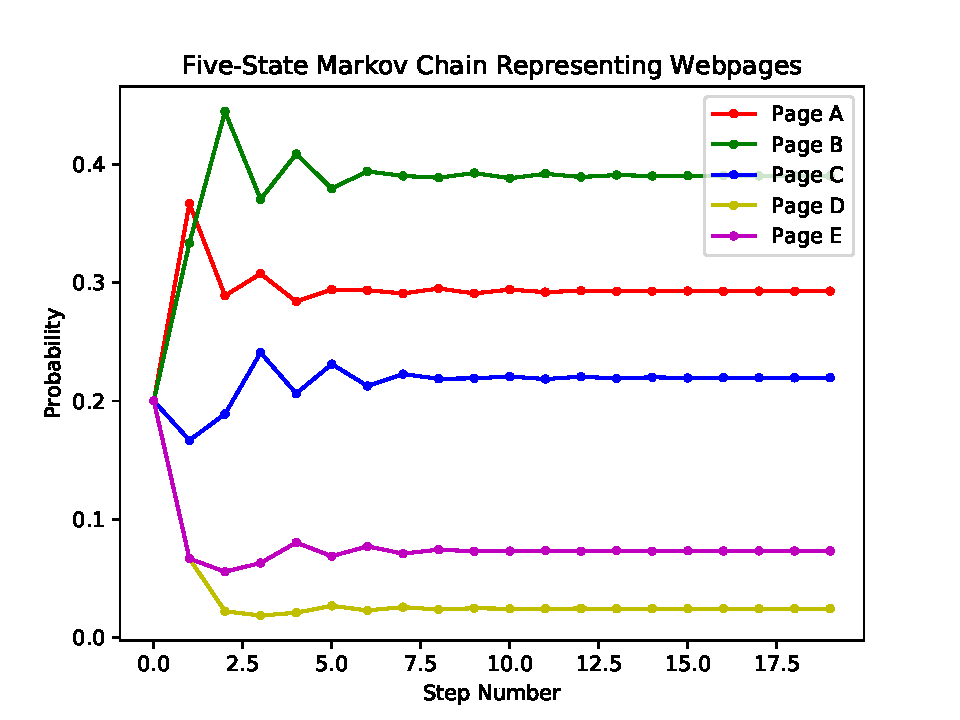
\includegraphics[width=0.49\textwidth]{Images/Problem2Figure1}
    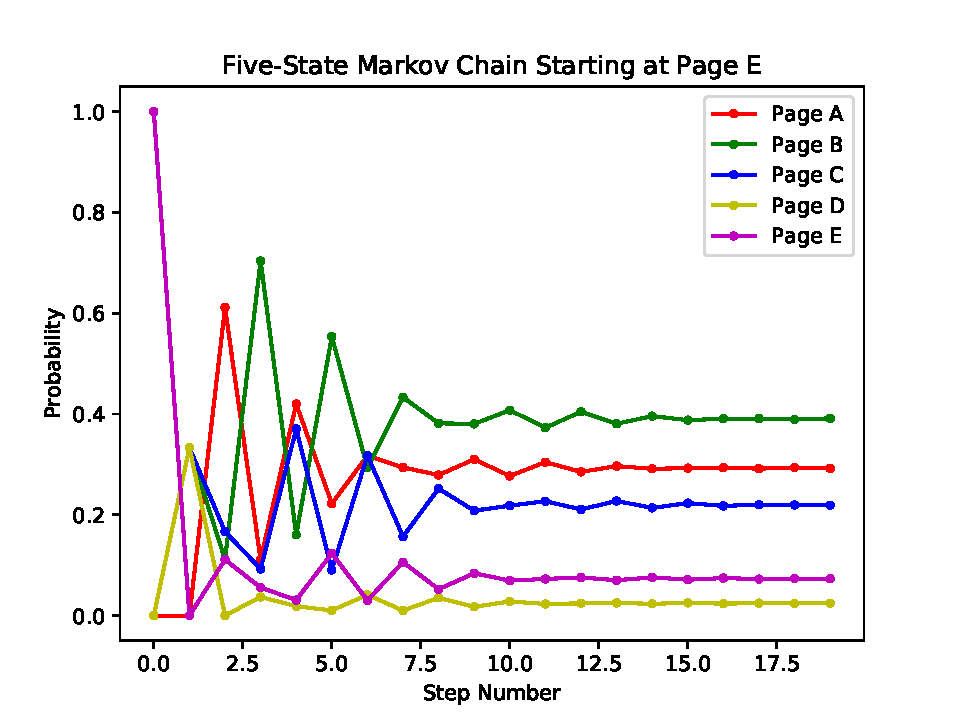
\includegraphics[width=0.49\textwidth]{Images/Problem2Figure2}
    \caption{Markov chain progressions.}
    \label{plot:google}
\end{figure}

\begin{table}[H]
    \begin{tabular}{|l|l|l|}
        \hline
        \multicolumn{3}{|l|}{Initial Probability Vector: \(v_1\)} \\ \hline
        Rank & Page & Probability Vector \\ \hline
        1 & B & \(1/5\) \\ \hline
        2 & A & \(1/5\) \\ \hline
        3 & C & \(1/5\) \\ \hline
        4 & E & \(1/5\) \\ \hline
        5 & D & \(1/5\) \\ \hline
    \end{tabular}
    \begin{tabular}{|l|l|l|}
        \hline
        \multicolumn{3}{|l|}{Initial Probability Vector: \(v_1\)} \\ \hline
        Rank & Page & Probability Vector \\ \hline
        1 & B & 0 \\ \hline
        2 & A & 0 \\ \hline
        3 & C & 0 \\ \hline
        4 & E & 0 \\ \hline
        5 & D & 1 \\ \hline
    \end{tabular}
    \caption{Probability vectors and page rankings.}
    \label{p2 table}
\end{table}

\section{Problem 3}
The purpose of this problem was to implement a ``drunkard's
walk''-type Markov chain where state \(i\) only leads to
state \(i+1\) and \(i-1\), and the first and last states
are absorbing states, meaning that they are ``inescapable.''
This was implemented with five states. Two ``walks,'' one
where the end state is 0 and one where the end state is 4,
are posted below. Note that the states never skip; i.e. they
only progress one state at a time.

\begin{figure}[H]
    \centering
    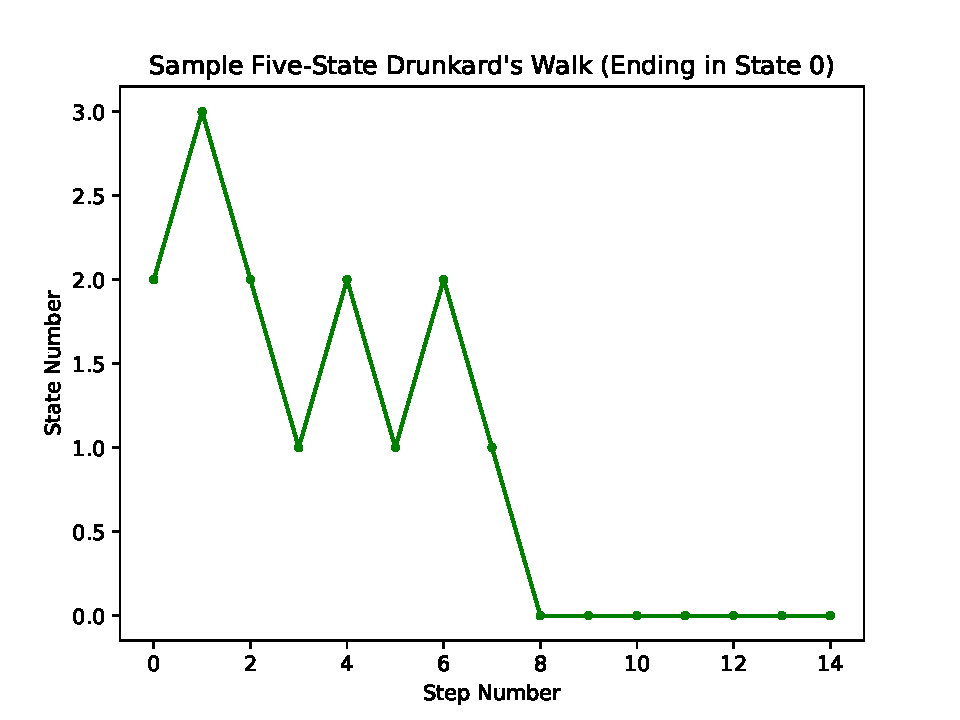
\includegraphics[width=0.49\textwidth]{Images/Problem3Figure2}
    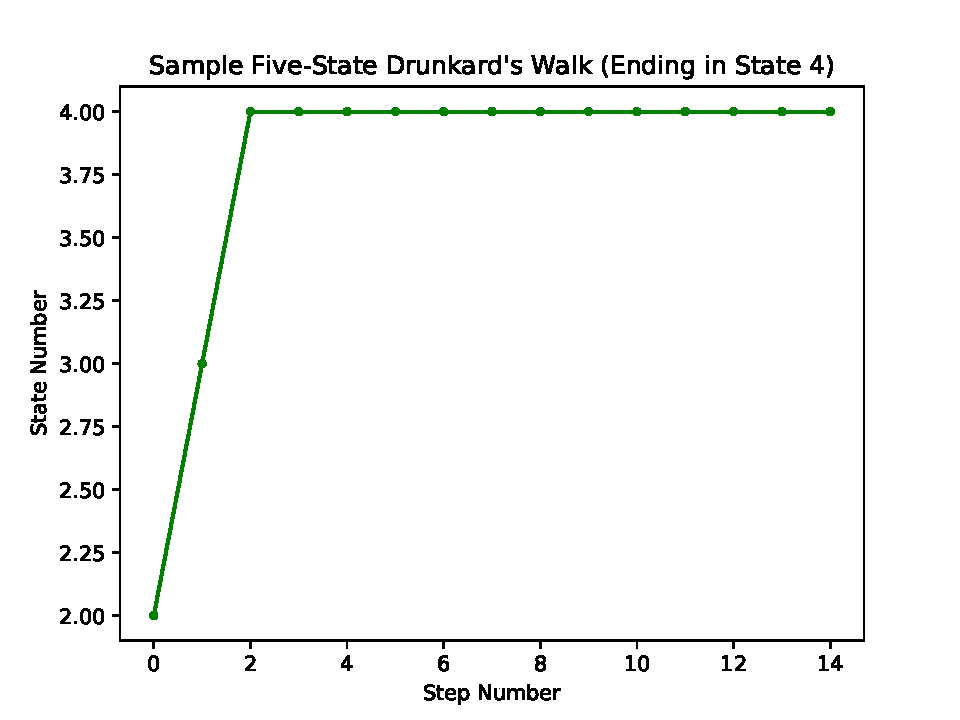
\includegraphics[width=0.49\textwidth]{Images/Problem3Figure3}
    \caption{Two walks.}
    \label{P3:walks}
\end{figure}

\section{Problem 4}
Figure \ref{P3:together} is a probability chart consisting
of \num{10000} walks. Note that State 1 and State 3 are
occupying the same space.

\begin{figure}[H]
    \centering
    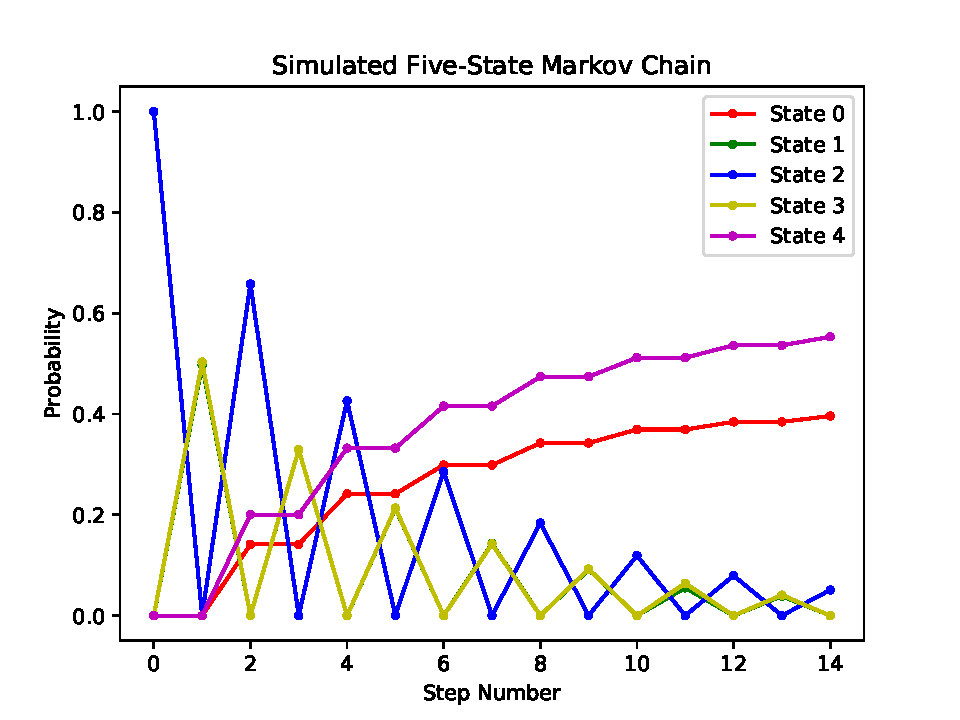
\includegraphics[width=\textwidth]{Images/Problem3Figure1}
    \caption{\num{10000} combined walks.}
    \label{P3:together}
\end{figure}

\begin{table}[]
    \begin{tabular}{|l|l|l|l|}
    \hline
    \multicolumn{4}{|l|}{Absorbtion Probabilities} \\ \hline
    \(b_{20}\) & 0.4 & \(b_{24}\) & 0.5 \\ \hline
    \end{tabular}
\end{table}

\end{document}
P[0] = np.array([[0, 1, 0, 0, 0], # Page A
[1/2, 0, 1/2, 0, 0], # Page B
[1/3, 1/3, 0, 0, 1/3], # Page C
[1, 0, 0, 0, 0], # Page D
[0, 1/3, 1/3, 1/3, 0]]) # Page E
